\documentclass[12pt,letterpaper,english,bibliography=totocnumbered,abstract=on]{scrartcl}

\usepackage{indentfirst}
\usepackage{appendix}
\usepackage{fullpage}
%\usepackage{subfiles}
\usepackage[T1]{fontenc}
\usepackage[latin9]{inputenc}
\usepackage{color}
\usepackage{babel}
\usepackage{verbatim}
\usepackage[unicode=true,pdfusetitle,
bookmarks=true,bookmarksnumbered=false,bookmarksopen=false,
breaklinks=true,pdfborder={0 0 0},pdfborderstyle={},backref=false,colorlinks=true]
{hyperref}
\hypersetup{linkcolor=blue,citecolor=blue,urlcolor=blue}

\usepackage{booktabs}
\usepackage{multirow}
\usepackage{adjustbox}
\usepackage{threeparttable}
\usepackage[table]{xcolor}
\usepackage{csquotes}
\usepackage{soul} % for hiliting text: \hl
% old style is authoryear
\usepackage[backend=biber, style=numeric, maxbibnames=99]{biblatex}
\addbibresource{mylibrary.bib}
\addbibresource{CRB.bib}

\usepackage[disable]{todonotes}

% Prevent page breaks within paragraphs
% https://tex.stackexchange.com/questions/21983/how-to-avoid-page-breaks-inside-paragraphs
\widowpenalties 1 10000


\begin{document}
\titlehead{US Forest Service Forest Health Protection Grant Progess Report 1}
\title{Establishment of Self-sustaining Biological Control of Coconut Rhinoceros Beetle Biotype G in Micronesia}
\author{Aubrey Moore, University of Guam}
%\date{Submitted December 30, 2020\\Revised January 28, 2021}
\maketitle
\begin{description}	
	\item[GRANTEE:] Aubrey Moore, University of Guam 
	\item[GRANT YEAR:] 2020
	\item[GRANT NUMBER:] 20-DG-11052021-229
	\item[GRANT PROGRAM:] Forest Health Protection
	\item[GRANT EXPIRATION DATE:] 2021-05-30
	\item[DATES COVERED BY THIS REPORT:] 2020-06-17 through 2020-12-31
	\item[GRANT STATUS:] Active
\end{description}	

\begin{footnotesize}
	\todo{change url}
\url{https://github.com/aubreymoore/FY19-PPA-Report-1/raw/master/PPA19-report2.pdf}
\end{footnotesize}


\newpage{}
\tableofcontents{}

\newpage
\listoftodos

\newpage


\section{OBJECTIVES AND SPECIFIC ACTIVITIES} 

%List the objectives individually that were included in the grant narrative.  Under those objectives include specific activities that occurred during the report timeframes.   

\subsection{Objective 1:  Survey to Determine Background OrNV Incidence} 

Our lab currently uses CRB-G adults collected from pheromone traps as test animals in bioassays evaluating OrNV isolates as biocontrol agents under the assumption that the Guam beetle population contains only the CRB-G biotype and is free from OrNV infection. In 2019 we gained the capacity to perform PCR in our lab began testing these assumptions. PCR results indicated that field-collected beetles were all CRB-G, but 18% of these tested positive for OrNV.

Based on these results, the PI decided to suspend bioassays until we had conclusive evidence of OrNV infection in the Guam CRB-G population.  An experimental plan was developed and executed. One hundred beetles were collected from each of two trapping sites (Leo Palace Resort in Southern Guam and the UOG Ag. Expt. Stn. in northern Guam). Gut samples were obtained from these beetles and tested using PCR in our lab and also in Sean Marshall's lab at AgResearch New Zealand. In PCR results from both labs all beetles tested positive for CRB-G biotype and negative for OrNV infection. We suspect that previous OrNV positive tests were the result of lab contamination (not false positives). 

\subsection{Objective 2: Establish Sustainable CRB-G Biocontrol by Autodissemination of OrNV}

This objective was on hold during the reporting period, pending results of Objective 1.

\subsection{Objective 3: Establish Island-wide Monitoring Systems for CRB and Coconut Palm Health}

Two roadside video surveys of CRB damage on Guam have been completed (the first in October 2020 and the second in December 2020).  Video frames were automatically analyzed using custom-trained object detectors. For each coconut palm detected in a video frame, a damage index was assigned and v-shaped cuts to fronds were counted. Results of both surveys were made  publicly available as interactive web maps (see the outputs section).

Equipment and instructions for video roadside surveys were provided to Rota to assist in their management of CRB.

\clearpage
\section{OUTPUTS} 

%Each Output listed in your grant narrative addressed individually.
%
%1) Output 1: list the output and what was accomplished.
%2) Output 2: list the output and what was accomplished.
%3) Etc.
%
%If output includes positions funded: (who, how long, type of work)
%
%If output includes Acres treated, include target species, number of acres and location 
%
%If output includes Acres surveyed, include target species, number of acres and location 
%
%Description and dollar value of equipment purchased, 
%
%Number of personnel trained.  

Bimonthly automated roadside surveys of CRB damage on Guam have been initiated and results were made publicly available as interactive web maps (Figs. \ref{fig:webmap1} and \ref{fig:webmap2}). The proportion of coconut palms damaged by CRB increased significantly from 19.2\% in October 2020 to 21.5\% in December 2020 (p < 0.001; Fisher's exact test). 

\begin{figure}[p]
	\centering
	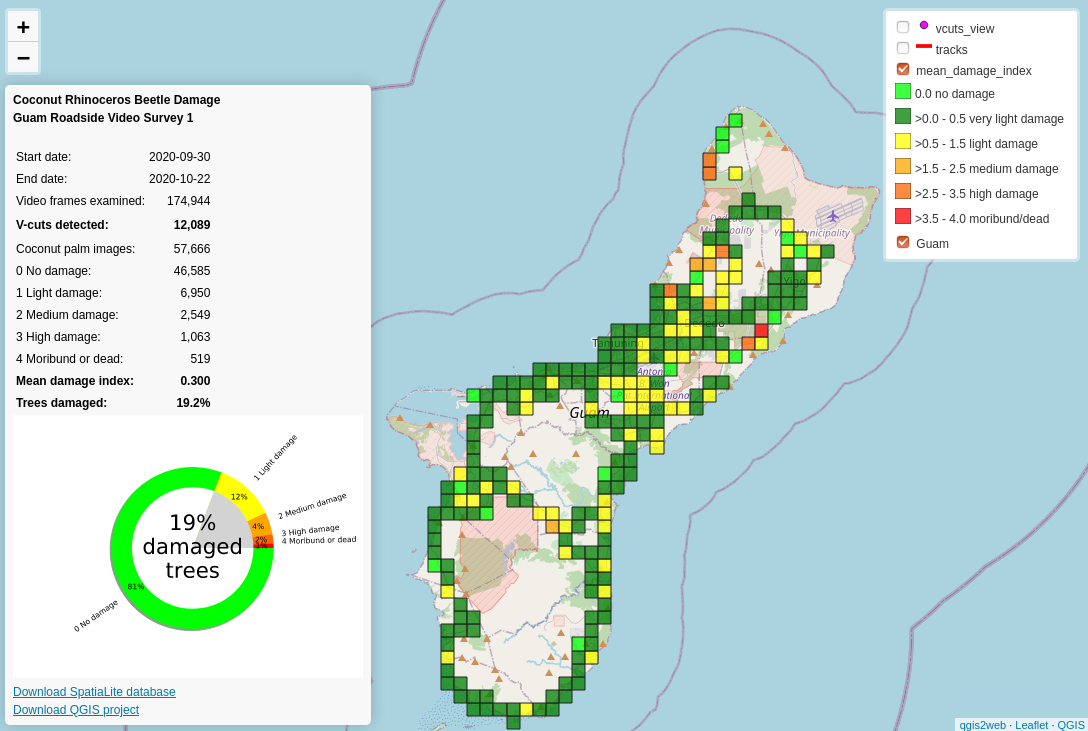
\includegraphics[width=0.75\linewidth]{images/crb-webmap-2020-10.png}
	\caption{Screenshot of an interactive web map of results from a roadside video survey of CRB damage on Guam in October 2020 URL: \url{https://aubreymoore.github.io/new-crb-damage-map}.}
	\label{fig:webmap1}
\end{figure}

\begin{figure}[p]
	\centering
	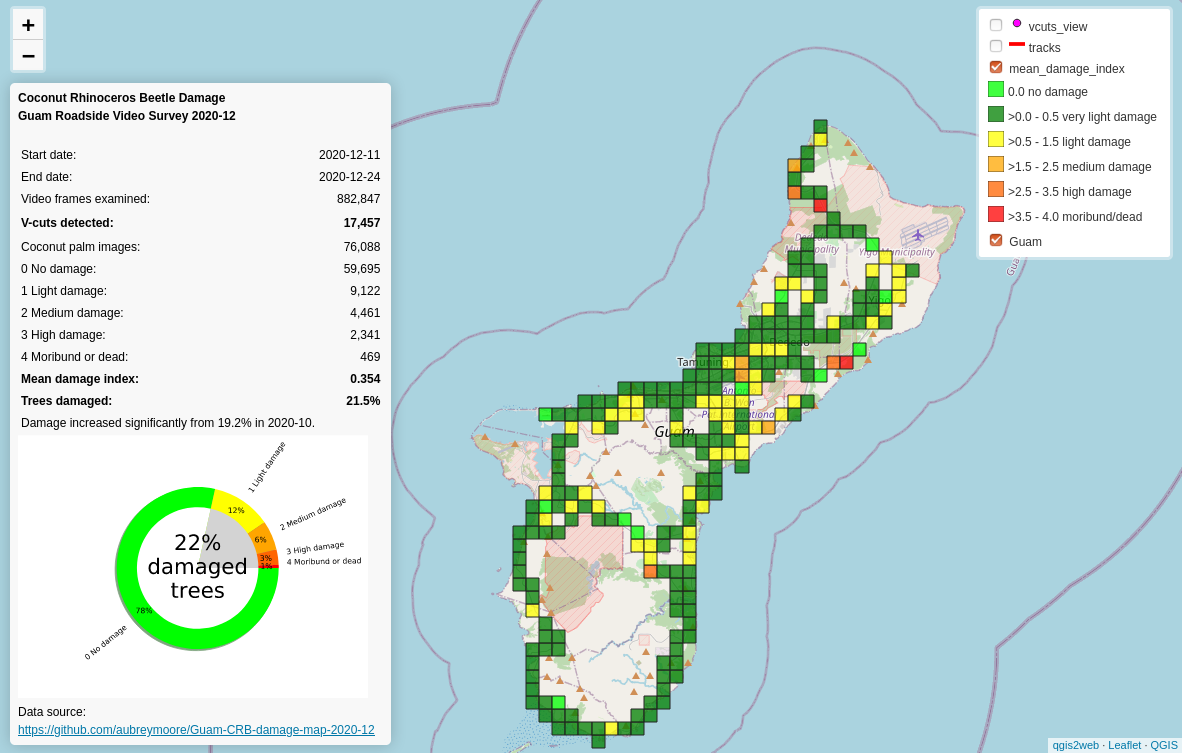
\includegraphics[width=0.75\linewidth]{images/crb-webmap-2020-12.png}
	\caption{Screenshot of an interactive web map of results from a roadside video survey of CRB damage on Guam in December 2020 URL: \url{https://aubreymoore.github.io/Guam-CRB-damage-map-2020-12/webmap/v1/}.}
	\label{fig:webmap2}
\end{figure}




\clearpage
\section{MONITORING \& EVALUATION}

%If post-treatment monitoring has been completed, provide the results, especially results that show effectiveness of treatments.  
%
%List any project evaluations that took place to determine whether goals and Statewide Strategies are being met.

Please see the Outputs section.

\section{BUDGET EXPENDITURES}

%Include budget table showing the expenditures (Personnel/salary costs, supplies purchased, contracts, etc.) that occurred during the reporting period

Progress during this reporting period was funded by alternate sources.

\medskip
\begin{tabular}{lrrl}
	\hline
	Category & Budget & Spent & Note \\
	\hline 
	Personnel & \$66,200 & \$0 & \\ 
	Benefits & \$14,720 & \$0 & \\ 
	Travel & \$4,000 & \$0 & \\
	Admin. fee & \$12,738 & \$0 & \\ 
	\hline 
\end{tabular} 



\section{PROBLEMS ENCOUNTERED THIS REPORTING PERIOD}

%Explain delays, adverse conditions or changed costs that significantly impair the ability to meet grant objectives.  If necessary, prepare a separate formal request for an extension of the grant period:

Progress on this project was impeded by COVID-19 travel restrictions which prevented collaborators from visiting Guam to participate in field work. Further delayed by delay was caused by Government of Guam \textit{stay at home} orders. The University of Guam was officially closed from March 20 to May 10 2020 and again from August 16 2020 to January 15 2021.


\section{CHANGES PLANNED}

% (If the scope of the objectives would change, or if more that 10\% of the total grant budget would change object class categories, prepare a separate formal request to amend the grant):

Nothing to report.


\section{CIVIL RIGHTS}

% - any activity that demonstrates Title VI compliance with civil rights requirements, such as documentation of outreach to underserved groups, public education documents in languages other than English, etc

Nothing to report.

\section{ATTACHMENTS}

% (photos of activities are very helpful, also electronic copies of survey and treatment maps, copies of developed brochures or posters, etc.):

None.

\section{PLANS}

% for work to be performed during next reporting period:

Nothing to report.

\end{document}
